\section{Physics}

\begin{Exercise}
Compute the lighting at position $P$ as seen from $E$. Take into account ambient, diffuse and specular lighting.
\begin{center}
  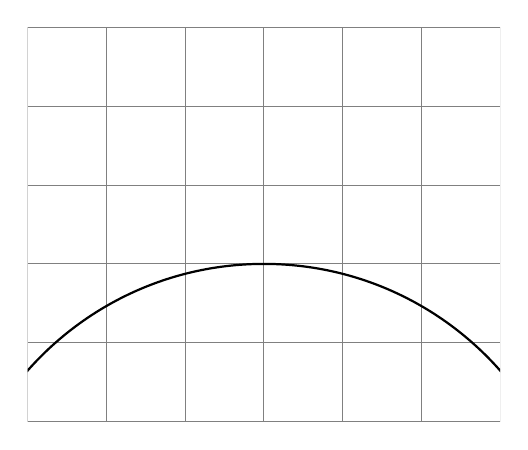
\begin{tikzpicture}
    \path[use as bounding box,clip] (-3,-2) rectangle (3,3);
    \draw[thin,gray] (-5,-5) grid (5,5);
    \coordinate (P) at (0,0);
    \coordinate (L) at (-1,2);
    \coordinate (E) at (2,1);
    \draw[thick] (0,-4) circle (4);
    \point[/point/label=P,/point/position=(P)]
    \point[/point/label=L,/point/position=(L)]
    \point[/point/label=E,/point/position=(E)]
  \end{tikzpicture}
\end{center}
\begin{center}
  \begin{tabular}{lcccc}
    & \textbf{r} & \textbf{g} & \textbf{b} \\
    \toprule
    light source & 1 & 1 & 0 \\
    ambient & 0.2 & 0.2 & 0.2 \\
    diffuse & 0.8 & 0.0 & 0.9 \\
    specular & 0.5 & 0.5 & 0.5 & e = 10
  \end{tabular}
\end{center}
\end{Exercise}


\begin{Exercise}
A sphere is centred at $C(3, 0, 0)$ and has radius $2$.
A ray of light starts at $P(2,2,2)$ and is directed straight towards
the sphere's centre. It hits the sphere at some position $H$.
The ray bounces off the sphere in a mirror-like way and proceeds to hit the YZ-plane at some point $Q$.
\begin{itemize}
  \item What are $H$'s coordinates?
  \item What is the reflected ray's direction?
  \item What are $Q$'s coordinates?
\end{itemize}
\begin{solution}
\[
  \begin{array}{rcl}
    H & = & \displaystyle \left(\frac{7}{3},\frac{4}{3},\frac{4}{3}\right) \\ \\
    N & = & \displaystyle \left(-\frac{1}{3},\frac{2}{3},\frac{2}{3}\right) \\ \\
    R & = & \displaystyle \left(-1,2,2\right) \\ \\
    Q & = & \displaystyle \left(0,6,6\right)
  \end{array}
\]
\end{solution}
\end{Exercise}

\begin{Exercise}
A light ray traverses a piece of glass.
\begin{center}
  \begin{tikzpicture}
    \draw[thick] (0,0) -- ++(0,2);
    \draw[thick] (5,0) -- ++(0,2);
    \draw[light] (-1,2) -- (0,1.5) -- (5,0.5) -- (6,0);

    \draw[|-|,thin] (0,-.5) -- ++(5,0) node[below,midway] {5};
    \draw[dashed,thin] (0,1.5) -- (6,1.5);
    \draw[dashed,thin] (5,0.5) -- (6,0.5);
    \draw[|-|,thin] (6.5,0.5) -- (6.5,1.5) node[right,midway] {x};

    \node at (-2,0) {air};
    \node at (2.5,0) {glass};
    \node at (7,0) {air};
  \end{tikzpicture}
\end{center}
\end{Exercise}
The direction of the light is $(2,-1)$, the thickness of the glass is 5. What is vertical distance travelled by the light ray, represented by $x$?


\begin{Exercise}
Below are a series of perfectly reflecting mirrors. A photon enters the scene.
What is its direction vector after the three bounces?
\begin{center}
  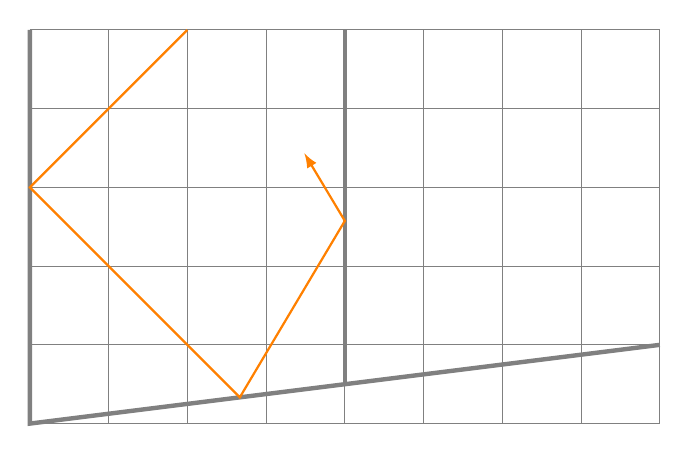
\begin{tikzpicture}
    \draw[thin,black!50] (0,0) grid (8,5);

    \draw[ultra thick,gray] (0,5) -- (0,0) -- (8,1);
    \draw[ultra thick,gray] (4,0.5) -- (4,5);

    \draw[orange,thick,-latex] (2,5) -- (0,3) -- (2.666,0.3333) -- (4,2.5744) -- ++(-0.514,0.858);
  \end{tikzpicture}
\end{center}
\begin{solution}
Original direction can be read from picture
\[
  \vec{v}_1 = (-1,-1)
\]
This vector does not need to be normalized. First mirror is vertical, hence its normal vector is
\[
  \vec{n}_1 = (1,0)
\]
The reflection formula assumes normal vectors have unit lengths, so we need to make
sure $\vec n_1$ has length $1$. After the first bounce, the photon's direction becomes
\[
  \vec v_2 = \vec v_1 - 2 \cdot (\vec v_1 \cdot \vec n_1) \cdot \vec n_1 = (1,-1)
\]
The second mirror is slightly tilted. Its normal vector is
\[
  \vec n_2 = (-1,8)
\]
We have to normalise this vector when using it in the reflection formula.
After the second bounce, the photon's direction is
\[
  \vec v_3 = \vec v_2 - 2 \cdot \left(\vec v_2 \cdot \frac{\vec n_2}{\norm{\vec n_2}}\right) \cdot \frac{\vec n_2}{\norm{\vec n_2}}
           = (0.723, 1.215)
\]
The third mirror has normal vector
\[
  \vec n_3 = (-1, 0)
\]
Bouncing the photon a third time gets us
\[
  \vec v_4 = (-0.723, 1.215)
\]
\end{solution}
\end{Exercise}

%%% Local Variables:
%%% mode: latex
%%% TeX-master: "model-exam"
%%% End:
